\documentclass[a4paper, notitlepage, abstracton]{scrartcl}
\usepackage[utf8]{inputenc}
\usepackage[italian]{babel}
\usepackage{fancyhdr}
\usepackage{lipsum}
\usepackage{float}

\usepackage{hyperref}
\usepackage{graphicx}
\usepackage{wrapfig}
\usepackage{listings}
\usepackage{float}
\usepackage{bytefield}
%\usepackage{fullpage}
\usepackage{algorithm}
\usepackage{algpseudocode}
\usepackage{amsmath}
\usepackage{todonotes}
\usepackage{tikz}

\usetikzlibrary{arrows,shapes}

\newcommand{\authorswe}{Davide Berardi, Matteo Martelli, Marco Melletti}

\pagestyle{fancy}
\rhead{Bajnarola}
\lhead{Progetto di sistemi distribuiti}

\rfoot{Davide Berardi, Matteo Martelli, Marco Melletti}
\lfoot{\thepage}
\cfoot{}
\renewcommand{\footrulewidth}{0.4pt}

\begin{document}

\title{Bajnarola}

\subtitle{Progetto di sistemi distribuiti}
\date{\today}

\pagenumbering{gobble}

\author{
	\begin{tabular}{c c c}
		Davide Berardi & Matteo Martelli & Marco Melletti\\
		0000712698     & 0000702472      & 0000699715
	\end{tabular}
}

\maketitle

\begin{abstract}
	Bajnarola e' un bel  gioco

\end{abstract}

\pagenumbering{arabic}

\section{Introduzione}
Sempre più giochi da tavolo ormai vantano una versione digitale,
caratterizzata dalla possibilità di permettere agli utenti di giocare in
modalità multiplayer.
Allo stesso tempo però sono ancora rare implementazioni distribuite di
giochi multiplayer le quali spesso sono invece basate su un architettura
client server. In questo documento descriveremo il nostro lavoro di
progettazione ed implementazione della versione software di un gioco da
tavolo con particolare interesse riguardo l'architettura di rete
distribuita utilizzata nella modalità multiplayer.

\subsection{Carcassone}
In particolare è stato nostro interesse occuparci del remake del gioco
da tavolo Carcassonne. Quest'ultimo nello specifico è un boardgame dei
primi anni 2000 basato su tessere che consiste nel creare un paesaggio medievale 
posizionando e accostando tra loro vari tipi di tessere, che rappresentano una parte di città, 
un tratto di strada, un campo o un monastero \footnote{Si fa riferimento
alla prima versione del gioco in cui non sono presenti fiumi}.
Completando quindi più città, strade, ecc, attraverso tali tessere, i
giocatori (previsti da 2 a 5) accumulano i punti necessari a vincere la partita.
Al fine di comprendere al meglio le prossime sezione di questo documento, 
vedremo
brevemente di seguito il funzionamento del gioco.
All'inizio della partita, una singola tessera è posizionata sul tavolo, scoperta; 
le altre tessere sono posizionate coperte nel mazzo e mischiate.
Ciascuna di tali tessere rappresenta un frammento di paesaggio, e può contenere uno o più dei seguenti elementi:

\begin{itemize}
	\item tratti di strada, inclusi incroci e curve
    \item aree cittadine racchiuse da mura
    \item campi che circondano le città e accolgono le strade
    \item un monastero
\end{itemize}

A turno, i giocatori estraggono una tessera dal mazzo e la posizionano scoperta sul tavolo
in contatto con le tessere già piazzate attraverso uno o più lati in modo coerente con le altre, 
in modo da proseguire eventuali strade, campi, o mura già presenti.

Dopo aver posizionato la tessera, il giocatore può decidere di piazzare
una pedina detta \emph{meeple} su di essa che reclama la proprietà di un elemento di terreno
 e non può essere piazzato su un elemento già reclamato da un altro
meeple. Può accadere comunque che un elemento possegga più di un
proprietario se diviene una congiunzione di due elementi dello stesso
tipo non precedentemente adiacenti.
Quando un elemento viene completato, se ad esempio le mura di una città

vengono chiuse o se una strada ha due estremità chiuse, il proprietario
di quell'elemento acquisisce i relativi punti. Il punteggio di un
elemento è dipendente dal numero e dal tipo di tessere che compongono
l'elemento.

Il gioco termina con il piazzamento dell'ultima tessera; vince il giocatore che ha totalizzato più punti.

Rimandiamo alla documentazione ufficiale di Carcassonne per ulteriori
dettagli.

La semplice struttura del gioco e la sua organizzazione a turni rende
interessante l'approccio distribuito in quanto si evita di incorrere in problemi 
di prestazioni tipici dei giochi reattivi. Quest'ultimi infatti %TODO
%vogliono bassa latenza etc. etc. ma non nel nostro caso.


\section{Aspetti progettuali}
	Il gioco in questione e' stato realizzato nell'ottica di un sistema
	resistente ai guasti, come richiesto da progetto.\\
	Tale obiettivo e' stato raggiunto utilizzando le funzioni RMI del
	linguaggio di programmazione Java, la comunicazione e' stata configurata
	in modo da risultare allo stesso tempo sia robusta sia in grado di
	fornire reattivita' ai client del gioco,
	nonostante quest'ultimo non utilizzi uno schema in tempo reale.\\

\subsection{Il gioco}
\subsection{La comunicazione}

\section{Aspetti implementativi}



\subsection{Il desing pattern MVC}

\subsection{Implementazione dello schema di gioco}

\begin{figure}
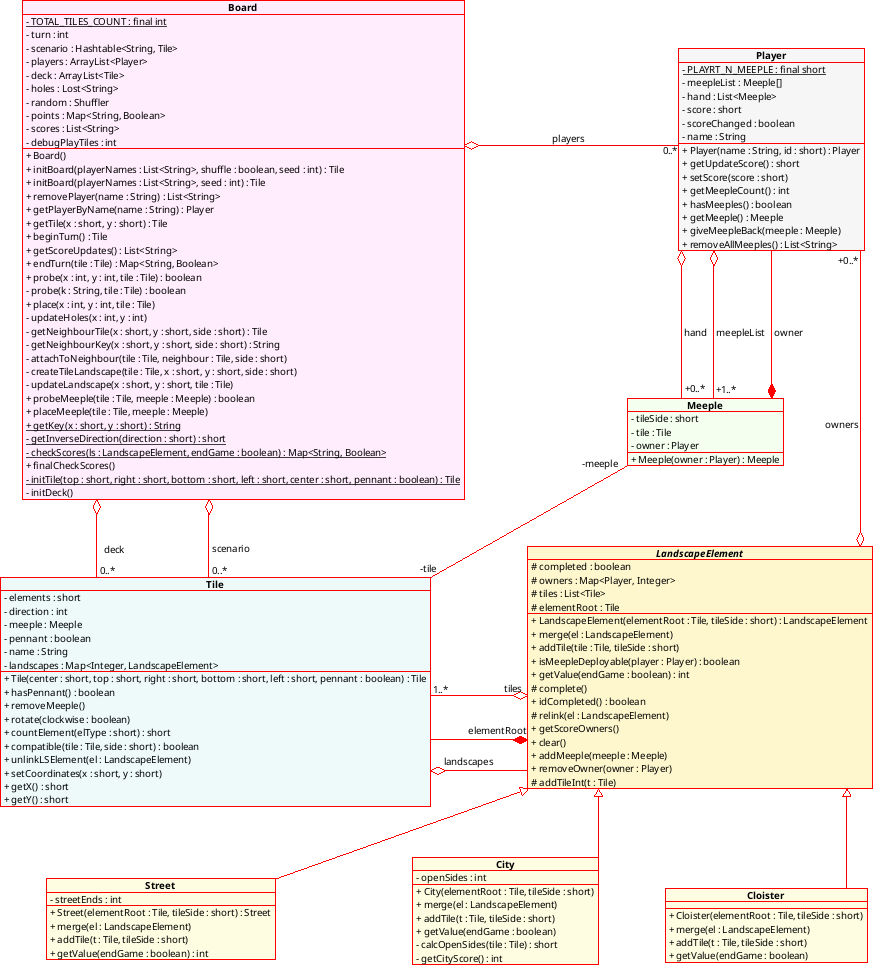
\includegraphics[width=\textwidth]{img/modelClassDiagram.png}
\end{figure}

\subsection{L'interfaccia grafica}
\subsection{La gestione e la distribuzione della rete}
	\subsubsection{Registrazione presso la lobby}
		Il primo passo svolto da ogni nodo di rete e' la registrazione
		presso un server centralizzato comune, implementante diverse
		"stanze" di gioco; le cosiddette lobby.\\
		Questo server aspettera' quindi la registrazione del numero
		specificato di partecipanti, inviando loro la lista dei
		giocatori per poi lasciare il pieno controllo
		ad essi, chiudendo la stanza.

% TODO struttura pacchetti???
\begin{figure}[H]
\begin{minipage}[t]{0.45\textwidth}
\centering
\begin{tikzpicture}[->,
	main node/.style={circle,draw,thick,fill=green!20,minimum size=4mm},
	lobby node/.style={ellipse,draw,thick,fill=blue!20,minimum size=4mm}
]
	\node[lobby node] (L) {Lobby Server};

	\node[main node, below of=L,xshift=-18mm,yshift=-5mm] (1) {1};
	\node[main node, below of=L,xshift=-7mm,yshift=-10mm] (2) {2};
	\node[main node, below of=L,xshift=7mm, yshift=-10mm] (3) {3};
	\node[main node, below of=L,xshift=18mm,yshift=-5mm] (4) {4};

	\draw[->] (1) to[bend left=10] (L);
	\draw[->] (L) to[bend left=10] (1);

	\draw[->] (2) to[bend left=10] (L);
	\draw[->] (L) to[bend left=10] (2);

	\draw[->] (3) to[bend left=10] (L);
	\draw[->] (L) to[bend left=10] (3);

	\draw[->] (4) to[bend left=10] (L);
	\draw[->] (L) to[bend left=10] (4);
\end{tikzpicture}
\caption{\scriptsize Registrazione presso il server lobby}
\end{minipage}
\begin{minipage}[t]{0.45\textwidth}
\centering
\begin{tikzpicture}[->,
	main node/.style={circle,draw,thick,fill=green!20,minimum size=4mm},
	notacc node/.style={circle,draw,thick,fill=red!20,minimum size=4mm},
	lobby node/.style={ellipse,draw,thick,fill=blue!20,minimum size=4mm}
]
	\node[lobby node] (L) {Lobby Server};

	\node[main node, below of=L,xshift=-18mm,yshift=-5mm] (1) {1};
	\node[main node, below of=L,xshift=-7mm,yshift=-10mm] (2) {2};
	\node[main node, below of=L,xshift=7mm, yshift=-10mm] (3) {3};
	\node[main node, below of=L,xshift=18mm,yshift=-5mm] (4) {4};

	\node[notacc node,below of=L,yshift=-18mm] (5) {5};

	\draw[->] (5) to[bend left=10] (L);
	\draw[->] (L) to[bend left=10] (5);

\end{tikzpicture}
\caption{\scriptsize Eccezione del server alla richiesta di una lobby chiusa}
\end{minipage}
\end{figure}

\subsubsection{Lo schema con leader dinamico.}
Lo schema di distribuzione si basa sull'elezione di un leader "dinamico", questo
leader e' deciso in base ad un lancio di un dado iniziale (nella realta'
implementato come un random intero a 32 bit, per evitare lanci ripetuti), questo
lancio viene quindi distribuito dai vari player ad ogni giocatore, creando un
\textbf{ordine} di gioco, il giocatore con punteggio maggiore verra' quindi
dichiarato come leader corrente, e da li a decrescere.\\
La topologia risulta quindi una rete monodirezionale con passaggio del
testimone (token ring) per la decisione del leader corrente.

\begin{figure}[H]
\begin{minipage}{.5\textwidth}
\centering
\begin{tikzpicture}[->,
	main node/.style={circle,draw,thick,fill=blue!20,minimum size=4mm},
	leader node/.style={circle,draw,thick,fill=green!20,minimum size=4mm}
]

	\def \n {5};
	\def \r {2.5cm};
	\def \m {8};

	\draw[->] (\m:\r) arc ({\m}:{360/\n -\m}:\r);

	\foreach \s in {2,...,\n} {
		\draw[->] ({360/\n * (\s-1) + \m}:\r) arc ({360/\n * (\s-1) + \m}:{360/\n * (\s) -\m}:\r);
		\node[main node] at ({360/\n * (\s-1)}:\r) {$\s$};
	}
	\node[leader node] at (0:\r) {1};
\end{tikzpicture}
\end{minipage}
\begin{minipage}{.5\textwidth}
\centering
\begin{tikzpicture}[->,
	main node/.style={circle,draw,thick,fill=blue!20,minimum size=4mm},
	leader node/.style={circle,draw,thick,fill=green!20,minimum size=4mm}
]

	\def \n {5};
	\def \r {2.5cm};
	\def \m {8};

	\draw[->,gray] (\m:\r) arc ({\m}:{360/\n -\m}:\r);

	\foreach \s in {2,...,\n} {
		\draw[->,gray] ({360/\n * (\s-1) + \m}:\r) arc ({360/\n * (\s-1) + \m}:{360/\n * (\s) -\m}:\r);
		\node[main node] at ({360/\n * (\s-1)}:\r) (\s) {$\s$};
	}
	\node[leader node] at (0:\r) (L) {1};

	\draw[->] (2) to[bend right=20] (L);
	\draw[->] (3) to[bend right=10] (L);
	\draw[->] (4) to[bend left=10] (L);
	\draw[->] (5) to[bend left=20] (L);
\end{tikzpicture}
\end{minipage}
\end{figure}

\subsubsection{Aggiornamenti allo stato}
	Uno degli aspetti piu' importanti del sistema di comunicazione del gioco
	e' la presenza di classi di differenza (classe \textbf{TurnDiff}), le
	suddette classi rendono la comunicazione il piu' leggero possibile
	essendo composte di:
	\begin{itemize}
		\item La rotazione della tessera posizionata;
		\item le coordinate della tessera;
		\item le posizioni relative del meeple se presente.
	\end{itemize}

\subsubsection{Tolleranza ai guasti}
	Il sistema risulta tollerante ai guasti di tipo crash.
	Nel caso di un guasto di tipo crash sul nodo leader corrente, sara' il
	sistema ad invocare un'eccezione di tipo \textbf{RemoteException} verso
	i nodi interroganti, che lo elimineranno quindi dalla loro lista di
	interrogazione, riconfigurando l'anello.\\
	Nel caso di un guasto di un nodo intermedio il risultato sara' il
	medesimo al momento di un'interrogazione da parte dei vari nodi
	dell'anello.\\
	Questo genere di configurazione mantiene coerente lo stato locale delle
	diverse istanze, poiche' ogni nodo aspetta la risoluzione delle varie
	mosse ad esso precedenti prima di essere interrogato a sua volta e poter
	agire.\\
	Questo schema e' banalmente possibile utilizzando una semplice rete di
	tipo token ring, ma e' stato scelto di implementare il tutto come una
	sorta di cricca per l'aggiornamento automatico e la visualizzazione dei
	risultati con latenze brevi: se si fosse ponderato per una struttura
	completamente circolare (utilizzante lo stesso modello logico) gli
	aggiornamenti allo stato locale sarebbero applicati solamente dopo che
	il controllo (e quindi la leadership) fosse tornata al nodo richiedente,
	risultando in un'attesa pari ad \textbf{N-1} turni; essendo il gioco
	in questione un gioco di logica non propriamente reattivo e con turni
	di gioco potenzialmente molto lunghi e riflessivi e' stato optato
	per un modello piu' pesante da un punto di vista
	di scambio di informazioni che da un punto di vista piu' leggero come
	comunicazioni ma, allo stesso tempo, meno reattivo per tutti i client.

\begin{figure}[H]
	\begin{minipage}{0.45\textwidth}
		\centering
\begin{tikzpicture}[->,
	main node/.style={circle,draw,thick,fill=blue!20,minimum size=4mm},
	crashed node/.style={forbidden sign,draw,thick,fill=red!50,minimum size=4mm}
]

	\def \n {5};
	\def \r {2.5cm};
	\def \m {8};

	\draw[->,gray] (\m:\r) arc ({\m}:{360/\n -\m}:\r);

	\foreach \s in {2,...,\n} {
		\draw[->,gray] ({360/\n * (\s-1) + \m}:\r) arc ({360/\n * (\s-1) + \m}:{360/\n * (\s) -\m}:\r);
		\node[main node] at ({360/\n * (\s-1)}:\r) (\s) {$\s$};
	}
	\node[crashed node] at (0:\r) (L) {1};

	\draw[->] (2) to[bend right=20] (L);
	\draw[->] (3) to[bend right=10] (L);
	\draw[->] (4) to[bend left=10] (L);
	\draw[->] (5) to[bend left=20] (L);
\end{tikzpicture}
	\end{minipage}
	\begin{minipage}{0.45\textwidth}
		\centering
\begin{tikzpicture}[->,
	main node/.style={circle,draw,thick,fill=blue!20,minimum size=4mm},
	crashed node/.style={circle,draw,thick,fill=gray,minimum size=4mm},
	leader node/.style={circle,draw,thick,fill=green!20,minimum size=4mm}
]

	\def \n {5};
	\def \r {2.5cm};
	\def \m {8};


	\draw[->,gray] ({360/\n * (2-1) + \m}:\r) arc ({360/\n * (2-1) + \m}:{360/\n * (2) -\m}:\r);
	\node[leader node] at ({360/\n * (2-1)}:\r) (2) {$2$};
	\draw[->,gray] ({360/\n * (3-1) + \m}:\r) arc ({360/\n * (3-1) + \m}:{360/\n * (3) -\m}:\r);
	\node[main node] at ({360/\n * (3-1)}:\r) (3) {$3$};
	\draw[->,gray] ({360/\n * (4-1) + \m}:\r) arc ({360/\n * (4-1) + \m}:{360/\n * (4) -\m}:\r);
	\node[main node] at ({360/\n * (4-1)}:\r) (4) {$4$};
	\node[main node] at ({360/\n * (5-1)}:\r) (5) {$5$};

	\draw[->,gray] (5) to [bend right=50] (2);

	\node[crashed node] at (0:\r) (L) {1};
	\draw[->] (3) to[bend right=10] (2);
	\draw[->] (4) to[bend left=10] (2);
	\draw[->] (5) to[bend left=20] (2);
\end{tikzpicture}
	\end{minipage}
\end{figure}

\section{Valutazione}
\lipsum

\section{Conclusioni}


\end{document}
